\documentclass[class=article,border=5pt,tikz]{standalone}
\usetikzlibrary{calc}

% define coordinates around a circle
% arg #1: radius of the circle, with default 1cm
% arg #2: number of coordinates around the circle
\newcommand{\chord}[2][1 cm]{
\pgfmathparse{#1/1 cm};
\edef\oc{\pgfmathresult cm};
  \foreach \i in {1,...,#2} {
    \coordinate (N\i) at (-\i*360/#2:#1);
    \draw (-\i*360/#2:\oc);
  }
}
% WARNING: dimension too large if #2 > 45

% command to draw an arc with given center, radius, angles
\def\centerarc[#1](#2)(#3:#4:#5)% Syntax: [draw options] (center) (initial angle:final angle:radius)
    { \draw[#1] ($(#2)+({#5*cos(#3)},{#5*sin(#3)})$) arc (#3:#4:#5); }
    
\begin{document}

% 6.28 * 1 = circumference, where r = 1
% 2*pi / 45 * 7 = 0.9773844 close to r = 1
% Ni to Ni+8 has length r (approx)

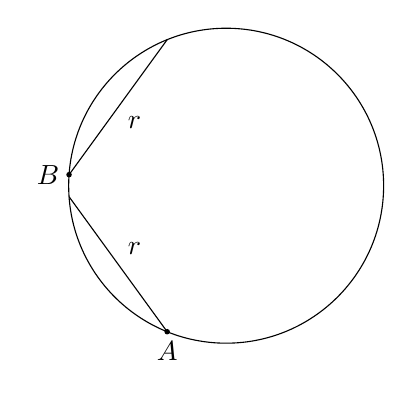
\begin{tikzpicture}[scale=2]
\chord[1 cm]{45} % create the coordinates
\draw (0,0) circle (1cm);
% first point
\node [below] at (N14) {$A$};
\fill (N14) circle (0.5pt);
\draw (N14) -- (N22) node [midway, above right] {$r$};
% second point
\node [left] at (N23) {$B$};
\fill (N23) circle (0.5pt);
\draw (N23) -- (N31) node [midway, below right] {$r$};
\end{tikzpicture}

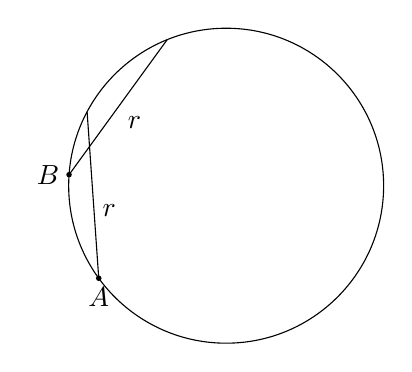
\begin{tikzpicture}[scale=2]
\chord[1 cm]{45} % create the coordinates
\draw (0,0) circle (1cm);
% first point
\node [below] at (N18) {$A$};
\fill (N18) circle (0.5pt);
\draw (N18) -- (N26) node [midway, below right] {$r$};
% second point
\node [left] at (N23) {$B$};
\fill (N23) circle (0.5pt);
\draw (N23) -- (N31) node [midway, below right] {$r$};
\end{tikzpicture}

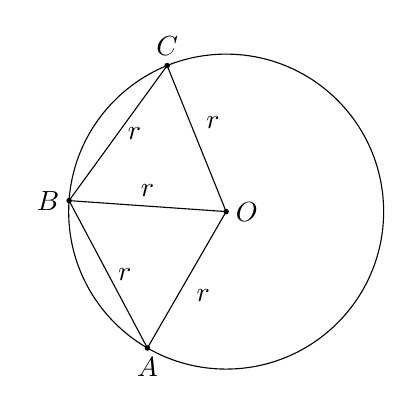
\begin{tikzpicture}[scale=2]
\chord[1 cm]{45} % create the coordinates
\draw (0,0) circle (1cm);
% first point
\node [below] at (N15) {$A$};
\fill (N15) circle (0.5pt);
\draw (N15) -- (N23) node [midway, right] {$r$};
% second point
\node [left] at (N23) {$B$};
\fill (N23) circle (0.5pt);
\draw (N23) -- (N31) node [midway, right] {$r$};
% third point
\node [above] at (N31) {$C$};
\fill (N31) circle (0.5pt);
% draw center and connecting radii
\node [right] at (0,0) {$O$};
\fill (0,0) circle (0.5pt);
\draw (0,0) -- (N23) node [midway, above] {$r$};
\draw (0,0) -- (N15) node [midway, below right] {$r$};
\draw (0,0) -- (N31) node [midway, above right] {$r$};
\end{tikzpicture}

% this figure unused
\begin{tikzpicture}[scale=2]
\chord[1 cm]{45} % create the coordinates
\draw (0,0) circle (1cm);
\draw [dashed] (0,0) -- (N44) node [midway, below] {$r$};
% first point
\node [below] at (N17) {$A$};
\fill (N17) circle (0.5pt);
% second point
\node [left] at (N23) {$B$};
\fill (N23) circle (0.5pt);
% arc of radius r centered on B
\centerarc[red](N23)(260:330:1)
\end{tikzpicture}

\end{document}
